%\documentclass{beamer}
\documentclass[handout]{beamer}

\usepackage{pgfpages} 

%\setbeameroption{show only notes}

\usetheme{default}

\mode<presentation> {
%  \usetheme{Warsaw}
  \usetheme{Frankfurt}
%  \usetheme{Boadilla}
%  \usetheme{Marburg}
}

\mode<handout>{\setbeamercolor{background canvas}{bg=black!5} %
    \pgfpagesuselayout{4 on 1}[letterpaper,border shrink=4mm,landscape] %
    \setbeameroption{show notes}}

\title[CAC High Performance Math] {High Performance Math}
\author{Brock Palen\\ \texttt{brockp@umich.edu}}
\date{TBD}

\begin{document}
  \setbeamercovered{transparent}  
  \begin{frame}
    \titlepage
    \url{http://cac.engin.umich.edu/training}
  \end{frame}

%table of contents
  \begin{frame}{Outline}
    \tableofcontents
  \end{frame}
 
\begin{frame}{References}
 \begin{block}{References}
  \begin{itemize}
   \item U.C. Berkeley CS267 Jim Demmel \\
     \url{http://www.cs.berkeley.edu/~demmel/cs267/}
   \item Numerical Algorithms Group     \\
     \url{http://www.nag.com/lapack-ex/}
   \item Basic Linear Algebra Subprograms \\
     \url{http://www.netlib.org/blas/}
   \item Linear Algebra Package         \\
     \url{http://www.netlib.org/lapack/}
  \end{itemize}
 \end{block}
 \note{
   All Training docs are available at \url{www.umich.edu/~brockp} \\
 } %end note
\end{frame} 



\section{Concepts}
\subsection{Terms}
\begin{frame}{Terms}
 \begin{block}{Terms}
  \begin{itemize}
   \item<1-> Bandwidth - Speed in GB/s of memory to CPU
   \item<2-> Floating Point Number - Floats and Doubles (1.2 5.002)
   \item<2-> Fixed Point Number - Ints (1 50 1,000)
   \item<3-> Floating Point Operation (Flop) - A mathematic operation on a floating point number
   \item<4-> Memory Reference - A call to memory for data
   \item<5->  $q=f/m$ - Ratio of Flops to References
   \item<6-> Cache - Fast memory local to the CPU
  \end{itemize}
 \end{block}
 \note{
  Most HPC applications require floating point calculations thus focus is on FLOPS and not fixed point performance. \\
  Data in cache is assumed to be latency free. It is also assumed to have enough bandwidth to feed the CPU.
 } %end note
\end{frame}
 \subsection {Memory vs CPU}
 \begin{frame}{CPU Speed}
  \begin{block}{CPU Performance}
   \begin{itemize}
    \item <1->Moore's Law
    \item <2->Focus and Rightly So
    \item <3->Multi-Core
    \item <4->Single Instruction Multiple Data (Vector)
   \end{itemize}
  \end{block}
  \note{
  \url{http://en.wikipedia.org/wiki/Moore's\_law} \\
  \url{http://en.wikipedia.org/wiki/SIMD}         \\
  \url{http://en.wikipedia.org/wiki/Vector\_processor} \\
  SIMD (SSE, 3DNow, AltiVec) is related to the vector CPU's systems like the NEC SX-9.  Vectors are for working on lists of numbers at the same time. It can be thought as a type of parallelism.  Most HPC Math Libraries make use of the SIMD unit on modern CPU's.  For example on the AMD Barcelona performance doubled in the SIMD (SSE 128) unit. \\
  SIMD is very related to GP-GPU processing and CPU's like the IBM Cell. \\
 
  Cell CPU (PS3 and Road Runner)\\ 
  \url{http://en.wikipedia.org/wiki/Cell\_microprocessor} \\
  Computed Unified Device Arch. GP-GPU for Nvidia Cards
  \url{http://en.wikipedia.org/wiki/CUDA}
  } %end note
 \end{frame}

 \begin{frame}{Memory Speed}
  \begin{block}{Memory Performance}
   \begin{itemize}
    \item <1-> Memory Size
    \item <2-> Memory Speed (GB/s) trails CPU Flops
    \item <3-> Memory Latency is Worse than You think
   \end{itemize}
  \end{block}
 \end{frame}
 \note{
  Memory speeds matter more than latency. Modern CPUs like the AMD Opteron have the memory controller right in the CPU. This lowers memory latency.  It also adds total bandwidth (speed in GB/s) for an entire system in an SMP system. In such systems memory needs to be balanced across CPU Sockets.  
 } %end note
 \begin{frame}{Human vs. Computer}
   \[
    \alpha A=C
   \]
  \begin{block}{xSCAL() Scale A Vector }
   \begin{itemize}
    \item<2-> n Flops
    \item<3-> 2n References
    \item<4-> q=1/2
    \item<5-> \alert{Memory must be faster than the CPU}
   \end{itemize}
  \end{block}
 \end{frame}
 \note{
   While using sequences of simple operations like $AB=c$ and $ \alpha B=c$ are simple for a human to have organized it is a very slow type of operation for a computer. Computers need opportunities for data reuse. \\
   BLAS 1 Functions: \\
   $AB=c$ is xDOT()  \\
   $\alpha B=c$ is xSCAL() \\
 These are the slowest of the BLAS operations.  Their ratio $ q=f/m $ is 2/3
 } %end note

\begin{frame}{Computers are Faster}
  \[ M[ \ddots ] A[\vdots] = B[\vdots]\]
 \begin{block}{xGEMV() Matrix Vector Multiplication}
  \begin{itemize}
   \item $ 2n^2 $ Flops
   \item $n^2+n $ References
   \item $q=2$
  \end{itemize}
 \end{block}
 \note{
   These are the BLAS 2 operations. They require that memory be half the speed of the CPU. We will see latter how in real world examples that because BLAS 2 (and BLAS 1) that there is not enough data reuse (none really) to allow the cache to keep the CPU fed.
 } % end note
\end{frame}

\begin{frame}{Computers are Faster Ctd.}
 \[ M[ \ddots ] N[ \ddots ] = C[ \ddots ] \]
 \begin{block}{xGEMM() Matrix Matrix Multiplication}
  \begin{itemize}
   \item $ 2n^3 \rightarrow n^3 $ Flops
   \item $ 4n^2 $ References
   \item $ q=n/2 $
  \end{itemize}
 \end{block}
\end{frame}
 \note{
  BLAS 3.  These calls are the basis of the LAPACK calls. Notice how as the size of M scales the ratio of flops (when coded right) increases to memory references.  The reason for this is clever coding can maximize reuse of data already requested from memory.  The vendor provided BLAS libs will cleverly make sure that the data for an upcoming flop is already in cache. \\
User coded routines for xGEMM() are really a serious of xGEMV() calls. These operations cause data to be requested redundantly from memory. \\
Users should always try to use BLAS 3 calls even when they could be done with BLAS 1 or 2.
 } % end note

\begin{frame}{BLAS 1 \& 2 performance}
\begin{center}
  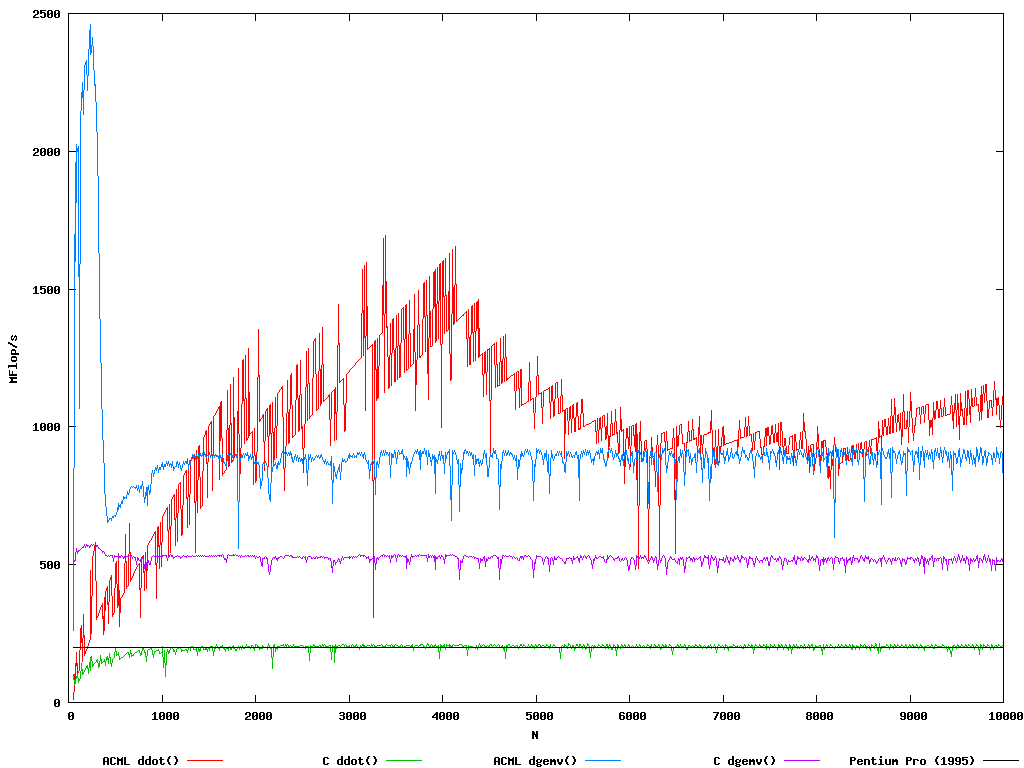
\includegraphics[height=3in]{blas12}
\end{center}
\note{
\begin{itemize}
 \item \texttt{pgcc -fastsse -DACML -DBLAS1 -DBLAS2 blasSpeeds.c -lacml -pgf90libs -lpgftnrtl}
 \item \texttt{pgi/7.2 acml/4.1.0}
 \item opt2218  2.613 Ghz, 2flop/Hz,  5.226 Gflop
 \item Pentium Pro 200 Mhz (1995) 1 FPU 200MFlop/s Peak
\end{itemize}
 
 The Pentium Pro released in 1995 was available up to 200MHz. This CPU consisted of a single FPU (Floating Point Unit) that could execute up to 1 FP op per Hz.  This resulted in a max performance of 1flop*200MHz=200MFlop/s.  
 The point of this example was to show how even simple operations most result in performance at some small fraction of peak performance. Of the C code presented only the matrix*vector results in speed faster than the Pentium Pro's peak.
} % end note
\end{frame}

\begin{frame}{BLAS 3}
\begin{center}
  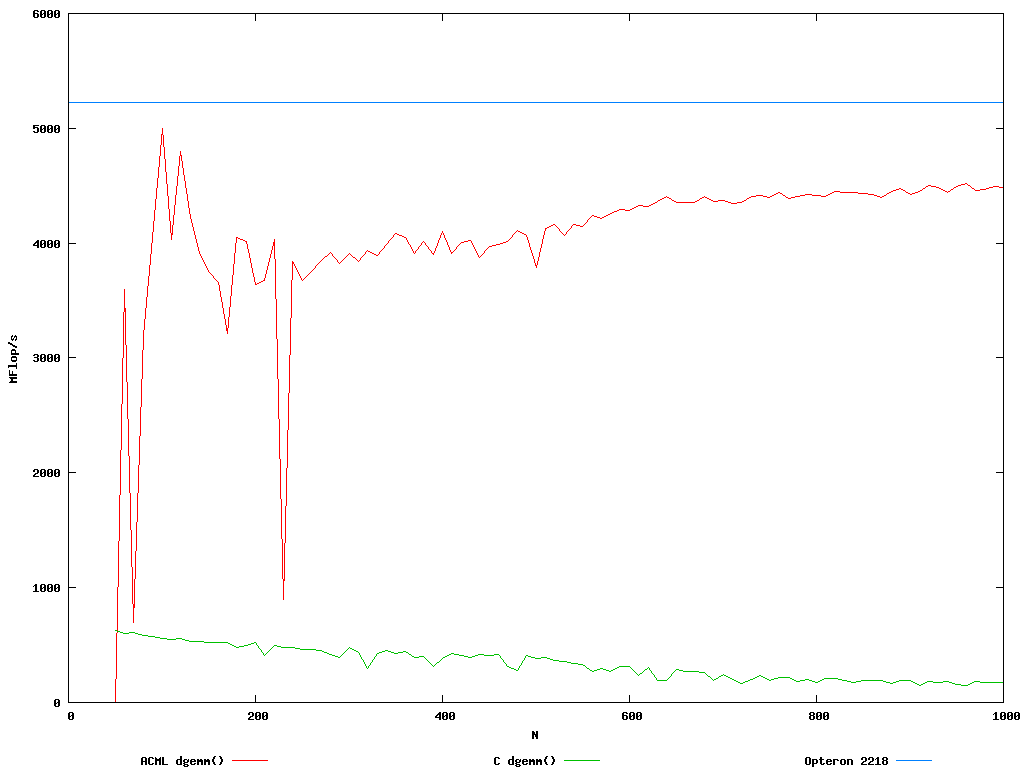
\includegraphics[height=3in]{blas3}
\end{center}
\note{
\begin{itemize}
 \item \texttt{pgcc -fastsse -DACML -DBLAS3 blasSpeeds.c -lacml -pgf90libs -lpgftnrtl}
 \item \texttt{pgi/7.2 acml/4.1.0}
 \item opt2218  2.613 Ghz, 2flop/Hz,  5.226 Gflop
\end{itemize}
BLAS3 allows maximum performance to be extracted from the CPU without any fancy programming.  The C code because it really is a matrix vector product over N vectors results in the same poor performance as BLAS2.  This example compares results on a Opteron 2218 with a peak speed of 5226 Mflop/s and the achieved speed. \\
Opteron 2218 has 2 FPU's and operates at 2.613 Ghz. 
} %
\end{frame}

\section{Formating}
\subsection{Types}
\begin{frame}{Types}
 \begin{block}{Type Prefix}
  \begin{itemize}
   \item D Double
   \item S Single/Float
   \item C Complex
   \item Z Double Complex
    \item<2-> SGEMM() vs ZGEMM()
  \end{itemize}
 \end{block}
 \note{
 BLAS Supports 4 types.  single, double, complex and double complex. A single letter D,S,C, or Z prefix a function for its use. For example DGEMM() is a matrix multiply when the matrices are made of doubles, while SGEMM() is for floats/REAL's.  \\
Note that Single should be faster than double and double faster than complex and complex faster than double complex. \\
Last C has no native complex type. Most the BLAS libs define a struct with real and imag parts. Check the header of your BLAS lib for their own complex type. Fortran uses the native complex and complex*16 types.

 }%note
\end{frame}

\subsection{Naming}
\begin{frame}{Naming}
 \begin{block}{Naming}
  \begin{columns}[T]
   \begin{column}{5cm}
    \begin{itemize}
     \item GE - GEneral
     \item SY - Symmetric
     \item HE - HErmitian
     \item TR - TRiangular
     \item GB - General Band
    \end{itemize}
   \end{column}
   \begin{column}{5cm}
    \begin{itemize}
     \item SB - Sym. Band
     \item HB - Herm. Band
     \item SP - Sum. Packed
     \item HP - Herm. Packed
     \item TP - Triang. Packed
    \end{itemize}
   \end{column}
  \end{columns}
 \end{block}
\end{frame}

\begin{frame}{Transpose and CBlas}
 \begin{block}{Transpose and CBlas options}
  \begin{itemize}
   \item 'N' - No Transpose, CblasNoTrans
   \item 'T' - Transpose, CblasTrans
   \item 'C' - Conjugate Transpose, CblasConjTrans
   \item 'U' or 'L' CblasUpper, CblasLower Triangular
   \item 'N' or 'U' CblasNonUnit, CblasUnit Triangular
  \end{itemize}
 \end{block}
 \begin{block}{CBlas Memory Ordering}
  \begin{itemize}
   \item CblasRowMajor
   \item CblasColMajor
  \end{itemize}
 \end{block}
 See: \url{http://www.netlib.org/blas/blasqr.ps}
\end{frame}

\section{Code}
\subsection{Obtaining}
\begin{frame}{Obtaining the BLAS}
\begin{block}{Libraries}
 \begin{itemize}
  \item Intel:  MKL Math Kernel Library 
  \item AMD: ACML AMD Core Math Library
  \item Apple/PowerPC/Intel: VecLib
  \item IBM/Power: ESSL
  \item Intel/AMD/Alpha/IA64: GOTO BLAS
  \item Any: ATLAS \url{http://math-atlas.sourceforge.net/}
 \end{itemize}
\end{block}
\note{
Each CPU manufacture publishes a library that implements the same functions. This allows code written on one system to compile and link against the BLAS lib for another system and extract all the performance of the new CPU type.  Also manufactures release updated versions of their BLAS libraries to use new CPU features. Because of this every time you are on a new system ask your Admin what CPU type it uses and grab the newest version of the BLAS library for that CPU. \\
Most are free, and some will run on others, for example ACML will work on Intel Chips. A wonderful library that is free and works on most if not all CPU's is ATLAS.
} %note
\end{frame}

\subsection{Support Code}
\begin{frame}{Fortran vs. C}
  \begin{center}
  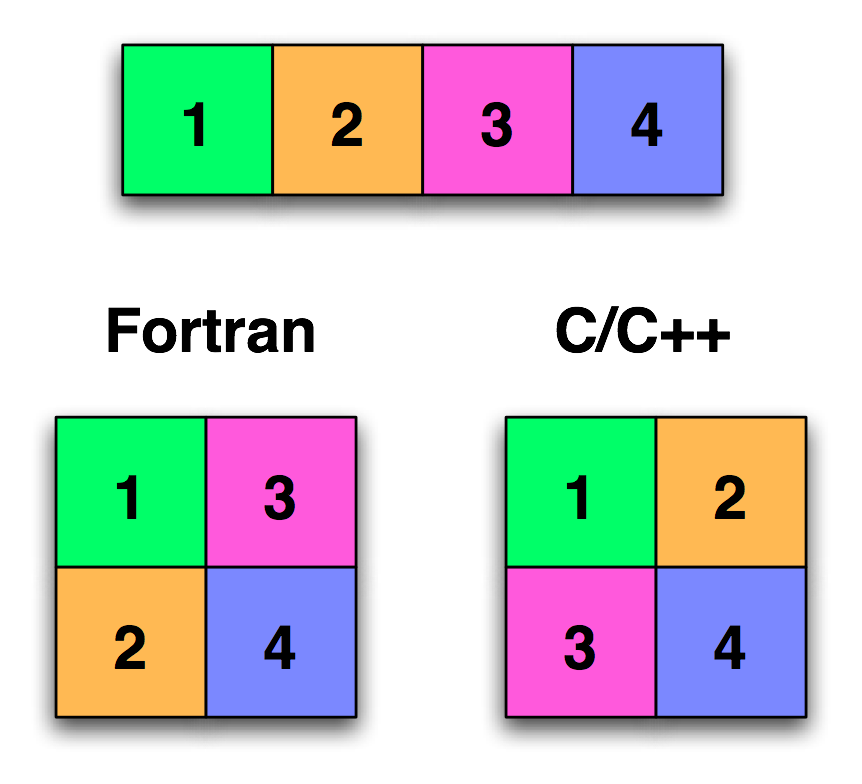
\includegraphics[height=3.0in]{matrixorder}  
  \end{center}
 \note{
 Fortran and C store matrices in memory two different ways.  C/C++ store them in row major. That is the fastest varying index is along the row of an array.  In Fortran it is column major. Because of this BLAS libraries that are based on Fortran (most of them) even their C calls expect the matrix to be in column major order. \\

Note for C/C++ code matrices can not be of the form M[i][j].  They must be of form M[i*j].  Fortran can use its normal form just fine M(j,i). \\

Fortran to C array conversion.\\
\begin{enumerate}
 \item Subtract 1 from each subscript
 \item Take the transpose
\end{enumerate}
 } %note
\end{frame}
\begin{frame}{Fortran vs. C}
 \begin{block}{Fortran from C}
 \begin{itemize}
  \item BLAS1 or any array does not require special treatment.
  \item A transposed matrix in C is a non-transposed matrix in Fortran:
  \begin{itemize}
   \item \texttt{dgemm('T', 'T', M, N, K, ALPHA, A, LDA, B, LDB, BETA, C, LDC);}
   \item \texttt{DGEMM('N', 'N', M, N, K, ALPHA, A, LDA, B, LDB, BETA, C, LDC)}
   \item When calling the Fortran based BLAS from C
  \end{itemize}
 \end{itemize}
 \end{block}
 \note{
 Because of the way Fortran stores data, a call from C is transposed in the view of the Fortran code that makes up the BLAS. To get around this a call to the BLAS only needs to told to work on the transpose of the input matrix. This is the same as saying DONT transpose from native Fortran.  Only C/C++ users need to worry about this. \\
A good alternative is the CBLAS which does most this work for you. The CAC will help anyone get there code to compile with the CBLAS.
 } % note
\end{frame}

\subsection{Free Performance}
\begin{frame}{Free Performance}
 \begin{block}{ACML 3.5.0 vs. 4.1.0}
  \begin{itemize}
   \item AMD Releases the Barcelona
   \item IBM Releases the CELL-BE
   \item Nvidia Releases CUBlas for GPU's
   \item <2-> Updating a BLAS library leverages new hardware
   \item <3-> Little or no code changes needed
  \end{itemize}
 \end{block}
 \note{
  Most major performance gains come from major changes in structure. To take advantage of these changes users would need to modify and recompile their code. A way a user can avoid this is by using a BLAS that was already built to take advantage of the new hardware. \\

Major Performance Changes:\\
\begin{itemize}
 \item Barcelona 128bit SIMD double peak speed/Hz
 \item CELL-BE reaches 102 Gflop/s using 8 SPE's \\
   \url{http://en.wikipedia.org/wiki/Cell\_(microprocessor)\#PowerXCell\_8i\_Variant}
 \item \$8,000 Tesla reaches 4 Tflop/s using GPU's \\
   \url{http://en.wikipedia.org/wiki/NVIDIA\_Tesla}
\end{itemize}
} %notes
\end{frame}
\begin{frame}{ACML 3.5.0 vs. 4.1.0}
 \begin{center}
   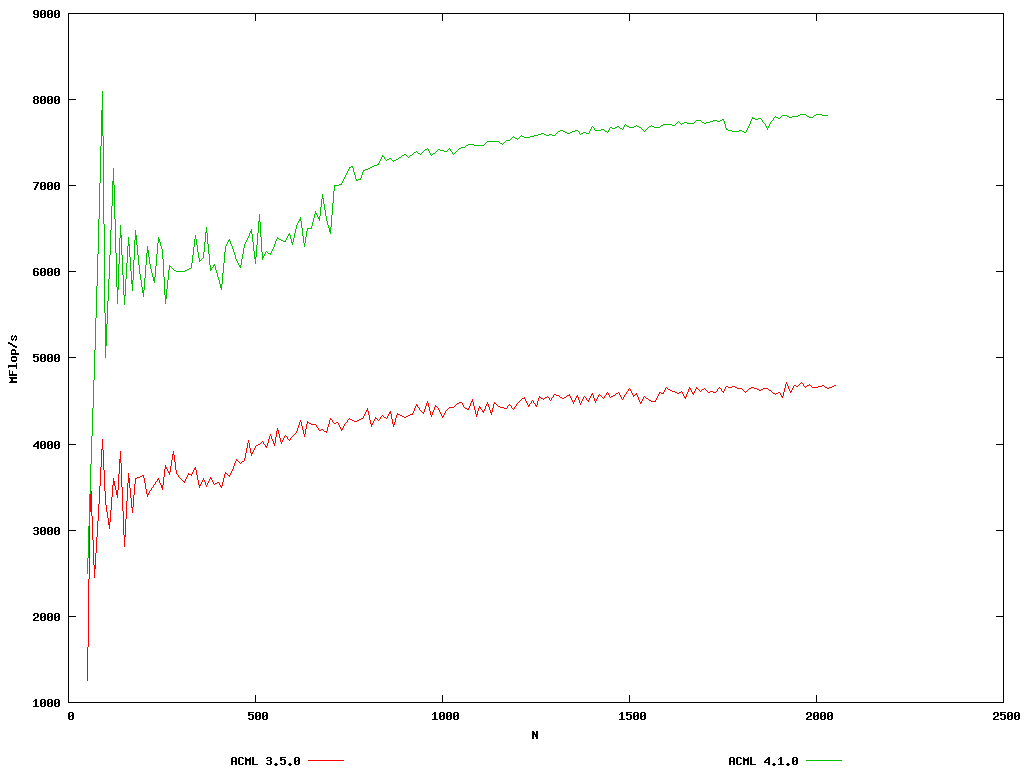
\includegraphics[height=3in]{blasVersions}
 \end{center}
 \note{
 Test was done on an AMD opt 2356 at 2311.87 MHz. \\
 This model of CPU added a 128 SIMD vector engine that doubles the available number of flops to code that uses it.  This boosted max speed from 4.62 Gflop/s to 9.24. The data for version 3.5.0 of the library was generated on the same physical node. \\

What users should take away is that using vendor BLAS lets old code get the maximum speed from available hardware.  As more and more exotic systems become available like GPU's and the CELL-BE this will ease performance upgrades to code.

} %
\end{frame}

\subsection{Free Parallel}
\begin{frame}{OpenMP and BLAS}
 \begin{block}{OpenMP}
  \begin{itemize}
   \item Type of Parallel Programming
   \item Shared Memory Parallel
   \item Simplest way to use Multi-Core
   \item Most BLAS has it built in
   \item Easy Performance 
  \end{itemize}
 \end{block}
 \note{
 OpenMP is one of the simplest forms of Parallel code. You can even mix in OpenMP libraries (BLAS) with code that is serial (my code).  OpenMP must live in a single node and was limited because of this till the advent of multi-core.  Most systems now have 8 cores and more on the way. \\
To compile code with OpenMP on make sure you are using the MP version of a library.  Enable OpenMP in your compiler and link again the MP BLAS: \\
\texttt{pgf90 -mp blascode.F90 -lacml\_mp -pgf90libs} \\
To set the number of threads/CPU's to use: \\
\texttt{export OMP\_NUM\_THREADS=8}

} %note
\end{frame}
\begin{frame}{OpenMP Performance}
 \begin{center}
  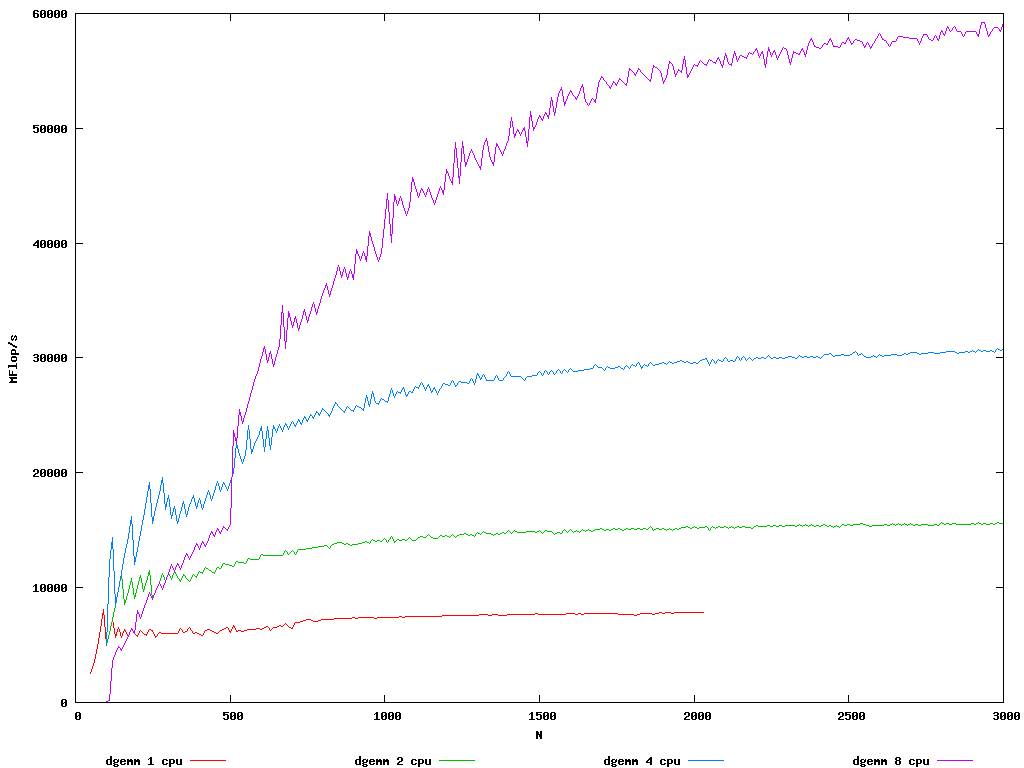
\includegraphics[height=3in]{openmp}
 \end{center}
 \note{
 Data generated with blasSpeed.c using acml/4.1.0-pgi pgi/7.2. CPU used was AMD Opteron 2356 at 2311MHz. \\
 Notice how for large data that the performance of DGEMM on 2 CPU's is twice as fast as 1 CPU.  4 is twice that of 2 and 8 twice as 4.  Note though that to reach peak speed on 8 cpus takes much larger data to reach peak performance. \\
Lastly users should remember that not all LAPACK functions use DGEMM and not all BLAS3 routines will reach the same speed as the same data size.
 } % note
\end{frame}

\section{Higher Level Libraries}
\subsection{LAPACK}
\begin{frame}{Linear Algebra Package}
 \begin{block}{LAPACK}
  \begin{itemize}
   \item Uses BLAS for performance
   \item Supports Parallel OpenMP via BLAS
   \item All Math Libraries provide it
   \item \url{http://www.netlib.org/lapack/}
   \item Simultaneous linear equations, least-squares solutions of linear systems of equations, eigenvalue problems, and singular value problems
   \item dgesv() Solve 20,000 equations in 2 minutes
  \end{itemize}
 \end{block}
 \note{
 \texttt{make dgesv} \\
 \texttt{./hdf-write}\\
 \texttt{./hdf-read} \\
 ACML/4.1.0 pgi/7.2, on 8 core opt 2356.
 } % note
\end{frame}
\begin{frame}{Summary}
 \begin{block}{Summary}
 \begin{itemize}
 \item News: \url{http://cac.engin.umich.edu}
   \begin{itemize}
    \item RSS feed
    \item New of changes, outages, other pertinent piece of information
   \end{itemize}
  \item Contact: \url{cac-support@umich.edu}
 \end{itemize}
 \end{block}
 \begin{block}{Survey}
    \url{https://www.engin.umich.edu/form/exit09}
 \end{block}
\end{frame}

\subsection{fftw}
\begin{frame}{Fastest Fourier Transform in the West}
 \begin{block}{fftw}
  \begin{itemize}
   \item \url{http://www.fftw.org}
   \item FFTW is a C subroutine library for computing the discrete Fourier transform (DFT) in one or more dimensions, of arbitrary input size, and of both real and complex data (as well as of even/odd data, i.e. the discrete cosine/sine transforms or DCT/DST). 
   \item Does support FORTRAN
   \item Works best on multiples of small primes
   \item Shared memory parallel via threads
   \item MPI Version
  \end{itemize}
 \end{block}
 \note{
 Free library works very well. Fftw is portable across most HPC systems. The newest version even supports the CellBE. Not as flexible as BLAS and LAPACK (not CPU vendor provided) but Fftw is the most portable high performance library available at no cost. \\
Good alternatives are each CPU vendors fft methods. MKL provides fft's for Intel CPUs, ACML does the same for AMD cpus.
} % note
\end{frame}

\subsection{Nag/IMSL}
\begin{frame}{NAG/IMSL}
 \begin{block}{Nag}
  \begin{itemize}
   \item \url{http://www.nag.com/numeric/numerical\_libraries.asp}
   \item Not free
   \item Built on BLAS for Performance
   \item SMP (Shared Memory Parallel) Version
   \item CAC Cluster has Nag Licenses
  \end{itemize}
 \end{block}
 \begin{block}{IMSL}
  \begin{itemize}
   \item \url{http://www.vni.com/products/imsl/}
   \item Not free
   \item Build on BLAS for Performance
   \item CAC Cluster has IMSL Licenses
  \end{itemize}
 \end{block}
\end{frame}

\section{Compile}
\subsection{ACML}
\begin{frame}{ACML Compile}
PGI ships ACML with their compiler: \\
\texttt{module load pgi/7.2}        \\
\texttt{pgf90 source.F90 -lacml}    \\
\texttt{pgcc  source.c -lacml -pgf90libs -lpgftnrtl} \\
Threaded OpenMP:                    \\
\texttt{pgf90 -mp source.F90 -lacml\_mp}            \\
\texttt{pgcc  -mp source.c   -lacml\_mp -pgf90libs -lpgftnrtl} \\
\texttt{export OMP\_NUM\_THREADS=4}                 \\
\end{frame}
\begin{frame}{ACML Compile (gfortran)}
\texttt{module load acml/4.0.1-gnu}       \\
\texttt{gcc source.c -I\$ACML\_INC -L\$ACML\_LINK -lacml -lgfortran} \\
\texttt{gfortran source.f -L\$ACML\_LINK -lacml}  \\
\begin{block}{Tips}
Versions also exists for \texttt{gfortran, ifort, pathscale, NAG, and SunStudio}for download from AMD. 
\end{block}
\begin{block}{Tools}
Example program \texttt{acmlVersion.c} will show which version of ACML linked against by calling \texttt{acmlversion()}
\end{block}
\end{frame}

\subsection{MKL}
\begin{frame}{MKL Compile}
\texttt{module load mkl}            \\
\texttt{ifort source.F90 -L \$MKL\_LINK -lmkl}      \\
\texttt{icc   source.c   -I \$MKL\_INC -L \$MKL\_LINK -lmkl}  \\
Threaded OpenMP:                    \\
Only need to set \texttt{OMP\_NUM\_THREADS} if not using OpenMP in your own code.  MKL always has threading enabled, \texttt{-openmp} is the flag to enable OpenMP in your own code.
\begin{block}{Tools}
Example program \texttt{mklVersion.c} will show which version of MKL is in use and linked against by calling \texttt{MKLGetVersion(*MKLVersion)} \\
\end{block}
\end{frame}

\subsection{CBlas}
\begin{frame}{CBlas}
\begin{block}{Building CBlas}
 CBlas can be built against any fortran BLAS library. This makes using BLAS much simpler from the C programers view. An example of how I build with CBlas requires that I link agains the BLAS library also.  This is nice because I can link ether serial BLAS or threaded BLAS.
\end{block}
\texttt{pgcc -mp source.c -I \$CBLAS\_INC -L \$CBLAS\_LINK -L \$ACML\_LINK -lcblas -lacml\_mp -pgf90libs -lpgftnrtl}       \\
\begin{block}{MKL VecLib and ATLAS}
There is no need to build CBlas against MKL, VecLib on the MAC, or ATLAS as it is already included.
\end{block}
\end{frame}
\end{document}
